\documentclass[11pt,a4paper]{article}

% Packages
\usepackage[utf8]{inputenc}
\usepackage[spanish, es-tabla, es-lcroman]{babel}
\usepackage{caption}
\usepackage{listings}
\usepackage{adjustbox}
\usepackage[shortlabels]{enumitem}
\usepackage{boldline}
\usepackage{amssymb, amsmath}
\usepackage[margin=1in]{geometry}
\usepackage{xcolor, color}
\usepackage{soul}
\usepackage{epstopdf}
\usepackage{hyperref}
\hypersetup{
     colorlinks   = true,
}

% Meta
\title{\textbf{ESTRUCTURA DE DATOS}\\
	   \textit{Práctica 1. Eficiencia de algoritmos}\\
	   \large \vspace{0.25em} Doble Grado de Informática y Matemáticas}
\author{Víctor Castro Serrano\\ Maximino Suárez van Gelderen}
\date{\today}

% Custom
\providecommand{\abs}[1]{\lvert#1\rvert}
\setlength\parindent{0pt}
\definecolor{Light}{gray}{.90}
\definecolor{mygreen}{rgb}{0,0.6,0}
\definecolor{mygray}{rgb}{0.5,0.5,0.5}
\definecolor{mymauve}{rgb}{0.58,0,0.82}
\renewcommand\labelenumi{(\emph{\roman{enumi})}}
\newcommand{\bm}[1]{\boldsymbol{#1}}

\lstset{literate=   % listings config
  {á}{{\'a}}1 {é}{{\'e}}1 {í}{{\'i}}1 {ó}{{\'o}}1 {ú}{{\'u}}1
  {Á}{{\'A}}1 {É}{{\'E}}1 {Í}{{\'I}}1 {Ó}{{\'O}}1 {Ú}{{\'U}}1
  {à}{{\`a}}1 {è}{{\`e}}1 {ì}{{\`i}}1 {ò}{{\`o}}1 {ù}{{\`u}}1
  {À}{{\`A}}1 {È}{{\'E}}1 {Ì}{{\`I}}1 {Ò}{{\`O}}1 {Ù}{{\`U}}1
  {ä}{{\"a}}1 {ë}{{\"e}}1 {ï}{{\"i}}1 {ö}{{\"o}}1 {ü}{{\"u}}1
  {Ä}{{\"A}}1 {Ë}{{\"E}}1 {Ï}{{\"I}}1 {Ö}{{\"O}}1 {Ü}{{\"U}}1
  {â}{{\^a}}1 {ê}{{\^e}}1 {î}{{\^i}}1 {ô}{{\^o}}1 {û}{{\^u}}1
  {Â}{{\^A}}1 {Ê}{{\^E}}1 {Î}{{\^I}}1 {Ô}{{\^O}}1 {Û}{{\^U}}1
  {œ}{{\oe}}1 {Œ}{{\OE}}1 {æ}{{\ae}}1 {Æ}{{\AE}}1 {ß}{{\ss}}1
  {ű}{{\H{u}}}1 {Ű}{{\H{U}}}1 {ő}{{\H{o}}}1 {Ő}{{\H{O}}}1
  {ç}{{\c c}}1 {Ç}{{\c C}}1 {ø}{{\o}}1 {å}{{\r a}}1 {Å}{{\r A}}1
  {€}{{\EUR}}1 {£}{{\pounds}}1 {ñ}{{\~{n}}}1
}

\lstset{    %listings config
  language=C++,
  belowcaptionskip=1\baselineskip,
  breaklines=true,
  frame=L,
  xleftmargin=0.5in,
  %otherkeywords={},
  showstringspaces=false,
  backgroundcolor=\color{white},
  basicstyle=\footnotesize\ttfamily,
  keywordstyle=\bfseries\color{purple!90!black},
  commentstyle=\itshape\color{gray!85!},
  identifierstyle=\color{blue!80!black},
  stringstyle=\color{green!60!black},
}

\newcommand\ddfrac[2]{\frac{\displaystyle #1}{\displaystyle #2}}

% Environments

\begin{document}
\maketitle

\section*{Condiciones de ejecución.}

Dado que en los siguientes ejercicios hablaremos de la eficiencia de distintos programas, conviene detallar las condiciones en las que se han llevado a cabo las pruebas. \\

\textbf{Hardware:} Asus GL552VW, Intel Core i5-6300HQ CPU @ 2.30GHz 4 cores, Intel HD Graphics 530 (Skylake GT2), 12GB RAM. \\
\textbf{Sistema Operativo:} Ubuntu 16.04.3 LTS 64-bit. \\
\textbf{Compilador:} g++ \\
\textbf{Opciones de compilación:} -O3 -o

\section*{Ejercicio 6.}

Compilando el algoritmo de la burbuja con la opción \textit{-O3} conseguimos que el compilador optimice el código de nuestro programa. Así, midiendo el tiempo de ejecución para distintos tamaños de vector y comparándolo con el que obtuvimos en el ejercicio 1, conseguimos la siguiente gráfica:

\begin{center}
	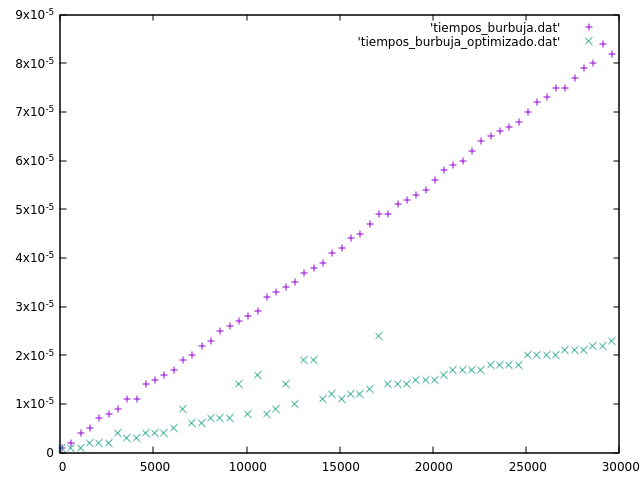
\includegraphics[height=7cm]{graf_comparacion.png}
\end{center}

Podemos observar claramente que el programa con las optimizaciones es mucho más rápido que sin ellas, como era de esperar.

\end{document}
